
Once we have accepted that some data sharing is going to happen, we have to also accept the need for the synchronization of concurrent accesses to the shared data. Remember that any concurrent access to the same data without such synchronization leads to data races and undefined behavior.

The most common way to guard shared data is with a mutex:

\begin{lstlisting}[style=styleCXX]
std::mutex m;
size_t count;// Guarded by m
… on the threads …
{
	std::lock_guard l(m);
	++count;
}
\end{lstlisting}

Here, we take advantage of the C++17 template type deduction for std::lock\_guard; in C++14, we would have to specify the template type argument.

Using mutexes is usually fairly straightforward: any code that accesses the shared data should be inside a critical section, that is, sandwiched between the calls to lock and unlock the mutex. The mutex implementation comes with the correct memory barriers to ensure that the code in the critical section cannot be moved outside of it by the hardware or the compiler (the compilers usually don't move the code across the locking operations at all, but, in theory, they could do such optimizations as long as they respect the memory barrier semantics).

The question that is usually asked at this point is, "How expensive is that mutex?" However, the question is not well defined: we can certainly give the absolute answer, in nanoseconds, for a particular piece of hardware and a given mutex implementation, but what does this value mean? It is certainly more expensive than not having a mutex, but without one, the program would be incorrect (and there are easier ways to make incorrect programs very fast). So, "expensive" can be defined only in comparison with the alternatives, which naturally leads to the question, what are the alternatives?

The most obvious alternative is to make the count atomic:

\begin{lstlisting}[style=styleCXX]
std::atomic<size_t> count;
… on the threads …
++count;
\end{lstlisting}

We also have to consider what memory order do we really need to be associated with operations on the count. If the count is later used to, say, index into an array, we probably need the release-acquire order. But if it's just a count, we just want to count some events and report the number, we have no need for any memory order restrictions:

\begin{lstlisting}[style=styleCXX]
std::atomic<size_t> count;
… on the threads …
count.fetch_add(1, std::memory_order_relaxed);
\end{lstlisting}

Whether we actually get any barriers or not depends on the hardware: on X86, the atomic increment instruction had the bidirectional memory barrier "built-in," and requesting the relaxed memory order is not going to make it any faster. Still, it is important to specify the requirement your code truly needs, both for portability and for clarity: remember that your real audience is not so much the compilers that have to parse your code but other programmers that need to read it later.

The program with the atomic increment has no locks and does not need any. However, it relies on a particular hardware capability: the processor has an atomic increment instruction. The set of such instructions is fairly small. What would we do if we needed an operation for which there are no atomic instructions? We don't have to go very far for an example: in C++, there is no atomic multiplication (and I don't know of any hardware that has such capability; certainly, it's not found on X86 or ARM or any other common CPU architecture).

Fortunately, there is a kind of "universal" atomic operation that can be used to build, with varying degrees of difficulty, any read-modify-write operation. This operation is known as compare-and-swap, or, in C++, as compare\_exchange. It takes two parameters: the first one is the expected current value of the atomic variable, and the second one is the desired new value. If the actual current value does not match the expected one, nothing happens, there is no change to the atomic variable. However, if the current value does match the expected one, the desired value is written into the atomic variable. The C++ compare\_exchange operation returns true or false to indicate whether the write did happen (true if it did). If the variable did not match the expected value, the actual value is returned in the first parameter. With compare-and-swap, we can implement our atomic increment operation in the following way:

\begin{lstlisting}[style=styleCXX]
std::atomic<size_t> count;
… on the threads …
size_t c = count.load(std::memory_order_relaxed);
while (!count.compare_exchange_strong(c, c + 1,
	std::memory_order_relaxed, std::memory_order_relaxed)) {}
\end{lstlisting}

Several notes are in order: first, the actual name of the operation in C++ is compare\_exchange\_strong. There is also compare\_exchange\_weak; the difference is that the weak version can sometimes return false even when the current and the expected values match (on X86, it makes no difference, but on some platforms, the weak version can result in a faster overall operation). Second, the operation takes not one but two memory order arguments: the second one applies when the compare fails (so it is the memory order for just the comparison part of the operation). The first one applies when the compare succeeds and the write happens.

Let us analyze how this implementation works. First, we atomically read the current value of the count, c. The incremented value is, of course, c + 1, but we cannot just assign it to the count because another thread could have incremented the count after we read it but before we update it. So we have to do a conditional write: if the current value of the count is still c, replace it with the desired value c + 1. Otherwise, update c with the new current value (compare\_exchange\_strong does that for us) and try again. The loop exits only when we finally catch a moment when the atomic variable did not change between the time we last read it and the time we're trying to update it. Of course, there is no reason to do any of this to increment the count when we have the atomic increment operation. But this approach can be generalized to any computation: instead of c + 1, we could use any other expression, and the program would work the same way. 

While all three versions of the code do the same operation, increment the count, there are fundamental differences between them that we must explore in more detail.

\subsubsubsection{6.3.1\hspace{0.2cm}Lock-based, lock-free, and wait-free programs}

The first version, with the mutex, is the simplest to understand: one thread can hold the lock at any time, so that thread can increment the count without any further precautions. Once the lock is released, another thread can acquire it and increment the count, and so on. At any time, at most one thread can hold the lock and make any progress; all remaining threads that need the access are waiting on the lock. But even the thread that has the lock is not guaranteed to proceed forward, in general: if it needs access to another shared variable before it can complete its job, it may be waiting on that lock, which is held by some other thread. This is the common lock-based program, often not the fastest, but the easiest to understand and reason about.

The second program presents a very different scenario: any thread that arrives at the atomic increment operation executes it without delay. Of course, the hardware itself must lock access to the shared data to ensure the atomicity of the operations (as we have seen in the last chapter, this is done by granting exclusive access to the entire cache line to one processor at a time). From the programmer's point of view, this exclusive access manifests itself as an increase in the time it takes to execute the atomic operation. However, in the code itself, there is no waiting for anything, no trying and retrying. This kind of program is called wait-free. In a wait-free program, all threads are making progress, that is, executing operations, at all times (although some operations may take longer if there is severe contention between threads for access to the same shared variable). A wait-free implementation is usually possible only for very simple operations (such as incrementing a count), but whenever it is available, it is often even simpler than the lock-based implementation.

It takes a bit more effort to understand the behavior of the last program. There are no locks; however, there is a loop that is repeated an unknown number of times. In this regard, the implementation is similar to the lock: any thread waiting on a lock is also stuck in a similar loop, trying and failing to acquire the lock. However, there is one key difference: in a lock-based program, when a thread has failed to acquire the lock and must try again, we can deduce that some other thread has the lock. We cannot be sure whether that thread is going to release the lock any time soon or that it, in fact, is making any progress toward completing its work and releasing the lock it holds (it may, for example, be waiting for a user to input something). In the program based on compare-and-swap, the only way our thread can fail to update the shared count is because some other thread updated it first. Therefore, we know that, of all threads trying to increment the count at the same time, at least one will always succeed. This kind of program is known as lock-free.

We have just seen examples of the three main types of concurrent programs:

\begin{itemize}
\item In a wait-free program, each thread is executing the operations it needs and is always making progress toward the final goal; there is no waiting for access, and no work needs to be redone.

\item In a lock-free program, multiple threads may be trying to update the same shared value, but only one of them will succeed. The rest will have to discard the work they have already done based on the original value, read the updated value, and do the computation again. But at least one thread is always guaranteed to commit its work and not have to redo it; thus, the entire program is always making progress, although not necessarily at full speed.

\item Finally, in a lock-based program, one thread is holding the lock that gives it access to the shared data. Just because it's holding the lock does not mean it's doing anything with this data, though. So, when the concurrent access happens, at most one thread is making progress, but even that is not guaranteed.
\end{itemize}

The difference between the three programs is clear, in theory. But, I bet every reader wants to know the answer to the same question: which one is faster? We can run each version of the code inside a Google benchmark. For example, here is the lock-based version:.

\hspace*{\fill} \\ %插入空行
\noindent
\textbf{01\_sharing\_incr\_mbm.C}
\begin{lstlisting}[style=styleCXX]
std::mutex m;
size_t count = 0;
void BM_lock(benchmark::State& state) {
	if (state.thread_index == 0) count = 0;
	for (auto _ : state) {
		std::lock_guard l(m);
		++count;
	}
}
BENCHMARK(BM_lock)->Threads(2)->UseRealTime();
\end{lstlisting}

The variables that must be shared between threads are declared at the global scope. The initial setup, if any, can be restricted to just one thread. Other benchmarks are similar; only the measured code changes. Here is the result:

\hspace*{\fill} \\ %插入空行
\begin{center}
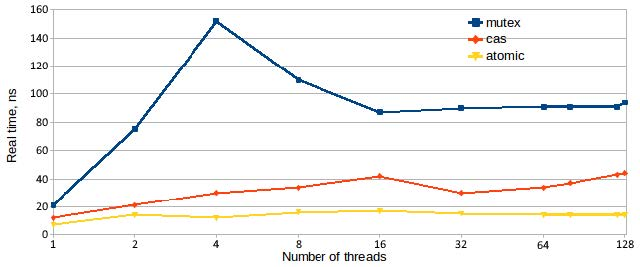
\includegraphics[width=0.9\textwidth]{content/2/chapter6/images/1.jpg}\\
Figure 6.1 – Performance of a shared count increment: mutex-based, lock-free (compare-and-swap, or CAS), and wait-free (atomic)
\end{center}

The only result that may be unexpected here is just how badly the lock-based version is performing. However, this is a data point, not the whole story. In particular, while all mutexes are locks, not all locks are mutexes. We can attempt to come up with a more efficient lock implementation (at least, more efficient for our needs).

\subsubsubsection{6.3.2\hspace{0.2cm}Different locks for different problems}

We have just seen that a standard C++ mutex performs very poorly when it is used to guard access to a shared variable, especially when there are many threads trying to modify this variable at the same time (if all threads were reading the variable, we would not need to guard it at all; concurrent read-only access does not lead to any data races). But is the lock inefficient because of its implementation, or is the problem inherent in the nature of the lock? From what we learned in the previous chapter, we can expect any lock to be somewhat less efficient than the atomically incremented counter simply because a lock-based scheme uses two shared variables, the lock and the count, versus just one, shared variable for an atomic counter. However, the mutexes provided by the operating system are usually not particularly efficient for locking very short operations such as our count increment.

The simplest and one of the most efficient locks for this situation is a basic spinlock. The idea of the spinlock is this: the lock itself is just a flag that can have two values, let's say 0 and 1. If the value of the flag is 0, the lock is not locked. Any thread that sees this value can set the flag to 1 and proceed; of course, the entire operation to read the flag and set it to 1 has to be a single atomic operation. Any thread that sees the value of 1 must wait until the value changes back to 0 to indicate that the lock is available. Finally, when a thread that changed the flag from 0 to 1 is ready to release the lock, it changes the value back to 0.

The code to implement this lock looks like this:

\begin{lstlisting}[style=styleCXX]
class Spinlock {
	public:
	void lock() {
		while (flag_.exchange(1, std::memory_order_acquire)) {}
	}
	void unlock() { flag_.store(0, std::memory_order_release); }
	private:
	std::atomic<unsigned int> flag_;
};
\end{lstlisting}

We show only the locking and unlocking functions in the code snippet; the class also needs the default constructor (an atomic integer is initialized to 0 in its own default constructor), as well as the declarations that make it non-copyable.

Note that locking the flag does not use a conditional exchange: we always write 1 into the flag. The reason it works is that, if the original value of the flag was 0, the exchange operation sets it to 1 and returns 0 (and the loop ends), which is what we want. But if the original value was 1, it is replaced by 1, that is, does not change at all.

Also, note the two memory barriers: locking is accompanied by the acquire barrier, while unlocking is done with the release barrier. Together, these barriers delimit the critical section and ensure that any code written between the calls to lock() and unlock() stays there.

You may be expecting to see the comparison benchmark of this lock versus the standard mutex, but we are not going to show it: the performance of this spinlock is terrible. To make it useful, it needs several optimizations.

First of all, note that if the value of the flag is 1, we don't actually need to replace it with 1, we can just leave it alone. Why does it matter? The exchange is a read-modify-write operation. Even if it changes the old value to the same value, it needs exclusive access to the cache line containing the flag. We don't need exclusive access to just read the flag. This matters in the following scenario: a lock is locked, the thread that has the lock is not changing it (it is busy doing its work), but all other threads are checking the lock and waiting for the value to change to 0. If they do not try to write into the flag, the cache line does not need to bounce between different CPUs: they all have the same copy of the memory in their caches, and this copy is current, no need to send any data anywhere. Only when one of the threads actually changes the value does the hardware need to send the new content of the memory to all CPUs. Here is the optimization we just described, done in code:

\begin{lstlisting}[style=styleCXX]
class Spinlock {
	void lock() {
		while (flag_.load(std::memory_order_relaxed) ||
		flag_.exchange(1, std::memory_order_acquire)) {}
	}
}
\end{lstlisting}

The optimization here is that we first read the flag until we see 0, then we swap it with 1. The value could have changed to 1 between the time we did the check and the time we did the exchange if another thread got the lock first. Also, note that, when pre-checking the flag, we don't care about the memory barrier at all since the final definitive check is always done using the exchange and its memory barrier.

Even with this optimization, the lock performs pretty poorly. The reason has to do with the way the operating systems tend to prioritize threads. In general, a thread that is doing heavy computing will get more CPU time on the assumption that it's doing something useful. Unfortunately, in our case, the most heavily computing thread is the one hammering on the flag while waiting for it to change. This can lead to an undesirable situation where one thread is trying to get the lock and has the CPU allocated to it, while another thread would like to release the lock but doesn't get scheduled for execution for some time. The solution is for the waiting thread to give up the CPU after several attempts, so some other thread can run and, hopefully, finish its work and release the lock.

There are several ways for a thread to release the control on the CPU; most are done by a system function call. There isn't a universal best way to do so. Experimentally, on Linux, a call to sleep for a very short time (1 nanosecond) by calling nanosleep() seems to yield the best results, usually better than a call to sched\_yield(), which is another system function to yield CPU access. All system calls are expensive compared to hardware instructions, so you don't want to call them too often. The best balance is achieved when we try to get the lock several times, then yield the CPU to another thread, then try again:

\hspace*{\fill} \\ %插入空行
\noindent
\textbf{01c\_spinlock\_count.C}
\begin{lstlisting}[style=styleCXX]
class Spinlock {
	void lock() {
		for (int i=0; flag_.load(std::memory_order_relaxed) ||
		flag_.exchange(1, std::memory_order_acquire); ++i) {
			if (i == 8) {
				lock_sleep();
				i = 0;
			}
		}
	}
	void lock_sleep() {
		static const timespec ns = { 0, 1 }; // 1 nanosecond
		nanosleep(&ns, NULL);
	}
}
\end{lstlisting}

The optimal number of attempts to acquire the lock before releasing the CPU will depend on the hardware and the number of threads, but generally, values between 8 and 16 work well.

Now we are ready for the second round of benchmarks, and here is the result:

\hspace*{\fill} \\ %插入空行
\begin{center}
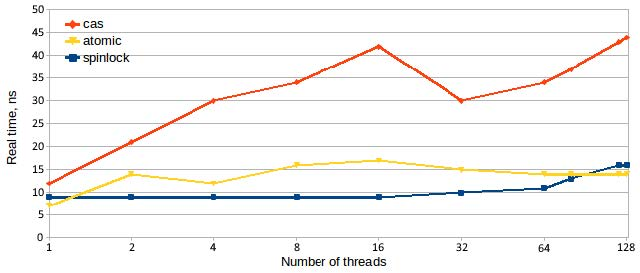
\includegraphics[width=0.9\textwidth]{content/2/chapter6/images/2.jpg}\\
Figure 6.2 – Performance of a shared count increment: spinlock-based, lock-free (compare-and-swap, or CAS), and wait-free (atomic)
\end{center}

The spinlock has done very well: it is soundly outperforming the compare-and-swap implementation and gives the wait-free operation tough competition. These results leave us with two questions: first, why don't all locks use spinlocks if they are so much faster? Second, why do we even need the atomic operations if the spinlock is so good (other than for implementing the lock, of course)?

The answer to the first question boils down to the title of this section: different locks for different problems. The downside of the spinlock is that the waiting thread continuously uses the CPU or is "busy waiting." On the other hand, the thread waiting on a system mutex is mostly idle (sleeping). Busy waiting is great if you need to wait for a few cycles, the duration of an increment operation: it's much faster than putting the thread to sleep. On the other hand, if the locked computation consists of more than a handful of instructions, the threads waiting on the spinlock waste a lot of CPU time and deprive the other working threads of access to the hardware resources they need. Overall, the C++ mutex (std::mutex) or the OS mutex is usually chosen for its balance: it's somewhat inefficient for locking a single instruction, it's OK for locking a computation that takes dozens of nanoseconds, and it beats the alternative if we need to hold the lock for a long time (long is relative here, processors are fast, so 1 millisecond is very long). Now, we are writing about extreme performance (and the extreme efforts to achieve it) here, so most HPC programmers either implement their own fast locks for guarding short computations or use a library that provides them. 

The second question, "Is there any other downside to the locks?" takes us to the next section.

\subsubsubsection{6.3.3\hspace{0.2cm}Lock-based versus lock-free, what is the real difference?}

When the conversation turns to the advantages of lock-free programming, the first argument is usually "it is faster." As we have just seen, this is not necessarily true: lock implementations can be very efficient if optimized for a particular task. However, there are other disadvantages that are inherent in the lock-based approach and do not depend on the implementation.

The first and the most infamous is the possibility of the dreaded deadlock. The deadlock occurs when the program uses several locks, let's say lock1 and lock2. Thread A has lock1 and needs to acquire lock2. Thread B already has lock2 and needs to acquire lock1. Neither thread can proceed, and both will wait forever because the only thread that can release the lock they need is itself blocked on a lock.

If both locks are acquired at the same time, the deadlock can be avoided if the locks are always acquired in the same order; C++ has a utility function for this purpose, std::lock(). However, often locks cannot be acquired at the same time: when thread A acquired lock1, there was no way to know that we will need lock2 as well since that information itself was hidden in the data that is guarded by lock1. We will see examples later in the next chapter when we talk about concurrent data structures.

If we cannot reliably acquire multiple locks, perhaps the solution is to try to acquire them, then, if we fail to get them all, release the locks we already hold so the other thread can get them? In our example, thread A holds lock1, it would try to get lock2 as well but without blocking: most locks have a try\_lock() call that either acquires the lock or returns false. In the latter case, thread A releases lock1 and tries to lock them both again. This might work, especially in a simple test. But it has a danger of its own: the livelock, when two threads constantly pass locks to each other: thread A has lock1 but not lock2, thread B has lock2, gives it up, gets lock1, now it can't get lock2 back because thread A has it. There are algorithms for acquiring multiple locks that guarantee success, eventually. Unfortunately, in practice, a long time may pass between now and eventually. These algorithms are also quite complex.

The fundamental problem of dealing with multiple locks is that the mutexes are not composable: there is no good way to combine two or more locks into one.

Even without the dangers of the livelock and the deadlock, lock-based programs suffer from other problems. One of the more frequent ones and one that is hard to diagnose is called convoying. It can happen with multiple locks or just one lock. Convoying looks like this: say we have a computation that is protected by a lock. Thread A currently has the lock and is doing its work on the shared data; other threads are waiting to do their part of the work. However, the work is not a one-shot deal: each thread has many tasks to do, and a part of each task requires exclusive access to the shared data. Thread A finishes one task, releases the lock, then zips through the next task until it gets to the point where it needs the lock again. The lock was released, any other thread can get it, but they are still waking up, whereas thread A is "hot" on the CPU. So, thread A gets the lock again simply because the competition is not ready for it. The tasks of thread A rush through the execution like trucks in a convoy, while nothing gets done on other threads. 

Yet another problem with locks is that they do not respect any notion of priority: a low-priority thread that is currently holding the lock will preempt any high-priority thread that needs the same lock. The high-priority thread thus has to wait for as long as the low-priority thread determines, the situation that seems entirely inconsistent with the notion of high priority. For this reason, this scenario is sometimes called priority inversion.

Now that we understand that the problems with locks are not limited to performance, let's see how a lock-free program would fare with regard to the same complications. First of all, in a lock-free program, at least one thread is guaranteed to not be blocked: in the worst-case scenario, when all threads arrive at a compare-and-swap (CAS) operation simultaneously and with the same expected current value of the atomic variable, one of them is guaranteed to see the expected value (since the only way it can change is via a successful CAS operation). All the remaining threads will have to discard their computation results, reload the atomic variable, and repeat the computation, but the one thread that succeeded on the CAS can move to the next task. This prevents the possibility of a deadlock. Without the deadlock and the attempts to avoid it, we do not need to worry about the livelock either. Since all threads are busy computing their way toward the atomic operation (such as CAS), the high-priority thread is more likely to get there first and commit its results, while the low-priority thread is more likely to fail the CAS and have to redo its work. Similarly, a single success in committing the results does not position the "winning" thread for any advantage over all the other threads: whichever thread is ready to attempt to execute CAS first is the one that succeeds. This naturally eliminates the convoying.

So, what's not to like about lock-free programming, then? Just two drawbacks, but they are major ones. The first is the flip side of its advantages: as we said, even the threads that fail their CAS attempts stay busy. This solves the priority problem, but at a very high cost: in the case of high contention, a lot of CPU time is wasted doing the work only to have it redone. Worse, these threads competing for access to the single atomic variable are taking away the CPU resources from other threads that are doing some unrelated computations at the same time.

The second drawback is of an entirely different nature. While most concurrent programs are not easy to write or understand, lock-free programs are incredibly difficult to design and implement correctly. A lock-based program just has to guarantee that any set of operations that constitutes a single logical transaction is executed under a lock. It gets harder when there are multiple logical transactions such that some, but not all, shared data is common to several different transactions. That is how we arrive at the problem of multiple locks. Still, reasoning about the correctness of a lock-based program is not that difficult: if I see a piece of shared data in your code, you must show me which lock guards this data and prove that no thread can access this data without acquiring this lock first. If this is not so, you have a data race, even if you haven't found it yet. If these requirements are met, you do not have data races (although you may have deadlocks and other problems).

Lock-free programs, on the other hand, have an almost infinite variety of data synchronization schemes. Since no thread is ever paused, we have to convince ourselves that, no matter the order in which the threads execute the atomic operations, the result is correct. Moreover, without the benefit of a clearly defined critical section, we have to worry about the memory order and the visibility of all the data in the program, not just the atomic variables. We have to ask ourselves, is there any way one thread can change the data, and the other thread can see the old version of it because the memory order requirements are not strict enough?

The usual solution to the problem of complexity is modularization and encapsulation. We collect the difficult code into modules where each one has a well-defined interface and a clear set of requirements and guarantees. A lot of attention is paid to the modules that implement various concurrent algorithms. This book takes you in a different direction: the rest of the chapter is dedicated instead to concurrent data structures.




































